\section{Results}\label{sec:results:krap}
Our results focused on adjusting three parameters: the number \k{} of nearest neighbors to consider, the \a{} threshold value, and the resolution algorithm.
\newcommand{\krapfigurewidth}{\linewidth}
\newcommand{\krapfigure}[1]{\includegraphics[height=0.50\textheight]{#1}}

\subsection{Adjusting \k{}}
Adjusting $k$ is an important first step. We investigate $k$ values ranging from 1 to 17, but focus primarily on $k \leq 12$. At this point, we do not filter the results in order to focus primarily on the affect of the size of the \knn{} list. Thus, $\alpha$ is 0, allowing for the full $k$ list to factor into classification.

\begin{figure}[t]
\centering
%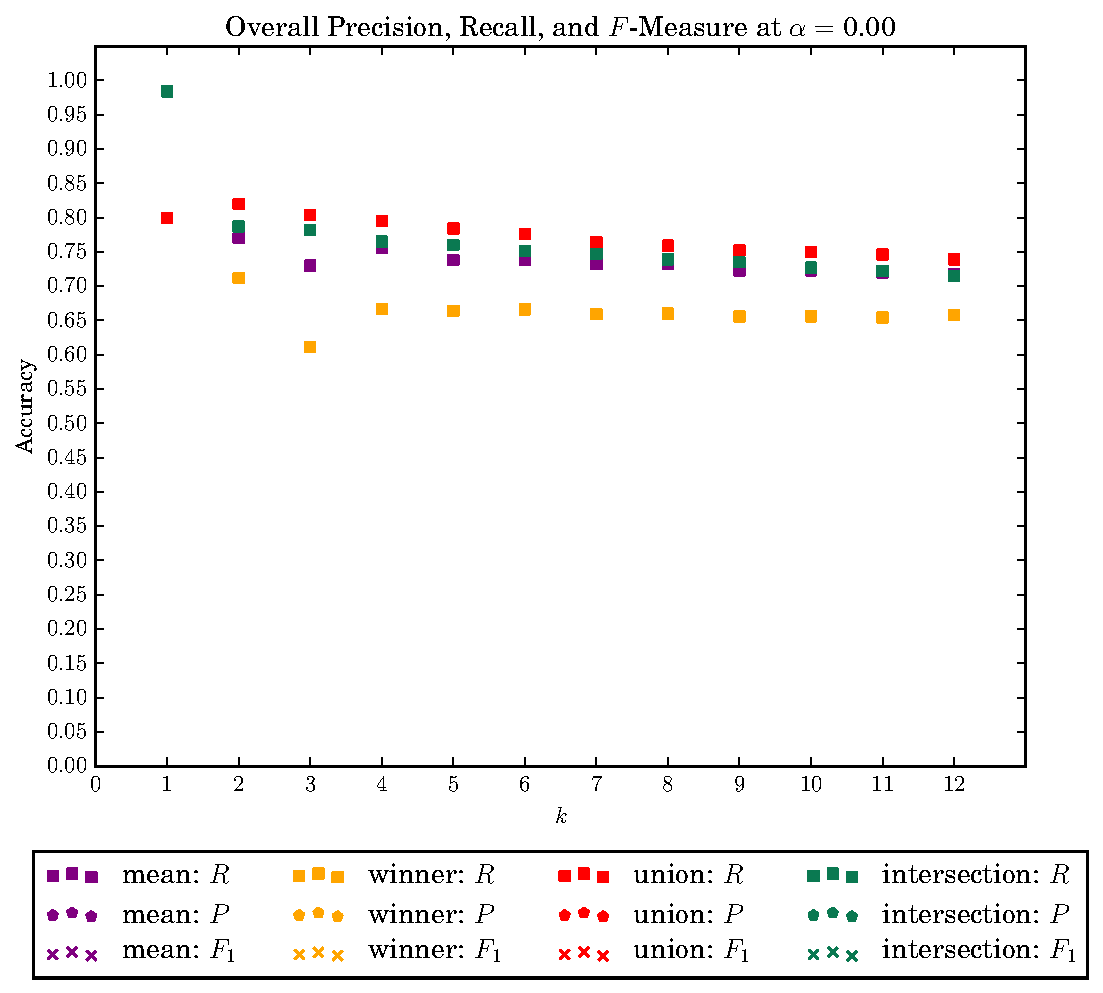
\includegraphics[width=3in]{figures/krap/Overall-ALL-metrics-12-0_000}
\krapfigure{figures/krap/Overall-ALL-metrics-12-0_000_new}
\caption{The accuracy  of all classifications performed with CPLOP across the four different algorithms with $\alpha=0.00$ shows little improvement for $k>5$. We look at only the percentage of correct classifications, since that value is equivalent to the precision and the recall.}
\label{fig:k_overall}
\end{figure}
Overall, for $k\geq5$, the accuracy does not improve, but instead levels off. Depending on the resolution algorithm, this value is between 65\% and 75\% accuracy, as shown in Figure \ref{fig:k_overall}. By ``overall,'' we mean that for every classification, we validated if it was correct and calculated what proportion to all classifications made that represents to determine accuracy. When looking at all classifications, precision and recall are identical values, as is $F$-measure.


\begin{figure}[t]
\centering
\krapfigure{figures/krap/Cow-ALL-metrics-12-0_000}
\caption{There are 1838 Cow \isol{}s in CPLOP. For most resolution algorithms, we observe little improvement when $k>5$.}
\label{fig:k_cow}
\end{figure}
One good example is the Cow. As Figure \ref{fig:k_cow} shows, Cow follows a trend similar to the overall accuracy, staying roughly between 70\% and 95\% accurate. Certain algorithms get worse for $k>5$, while other improve.

\begin{figure}[t]
\centering
\krapfigure{figures/krap/Cow-ALL-pvr-12-0_000}
\caption{There are 1838 Cow \isol{}s in CPLOP. Looking at the Recall as it compares to the Precision for $\alpha=0.99$ allows us to visualize the tradeoffs we make when picking a $k$ value. Labeled within each datapoint is the $k$ value at that point}
\label{fig:k_cow_pvr}
\end{figure}
Figure \ref{fig:k_cow_pvr} examines the relationship between $R$ and $P$. This can help us understand the trade offs of choosing one $k$ over another. We will later build a meaningful strategy for how confident we are at recalling a species versus our confidence in a classification of a species.


%ALPHA
\subsection{Adjusting \a{}}
By adding a threshold value, we investigated whether this further limitation improves the accuracy by restricting outliers from populating a \knn{} list. We investigate $\alpha = \{0.00,0.98,0.99\}$. Outside of this study, $\alpha = 0.99$ defines the boundary between strains. One reason we investigate 0.98 is to see whether loosening our definition of strain differentiation gives us a better accuracy.

\begin{figure}[t]
\centering
\krapfigure{figures/krap/Overall-ALL-metrics-12-[-0_----0_98--0_99]}
\caption{Shown is the accuracy of all classifications performed with CPLOP across the four different algorithms. We find that the accuracy of certain resolution algorithms perform better with higher $\alpha$ values.}
\label{fig:alpha_overall}
\end{figure}

Overall, we observe that the accuracy slightly improves as we increase the $\alpha$ threshold. Figure \ref{fig:alpha_overall} shows that overall, the accuracy increases as we increase $\alpha$. 

%\begin{figure}[t]
%\centering
%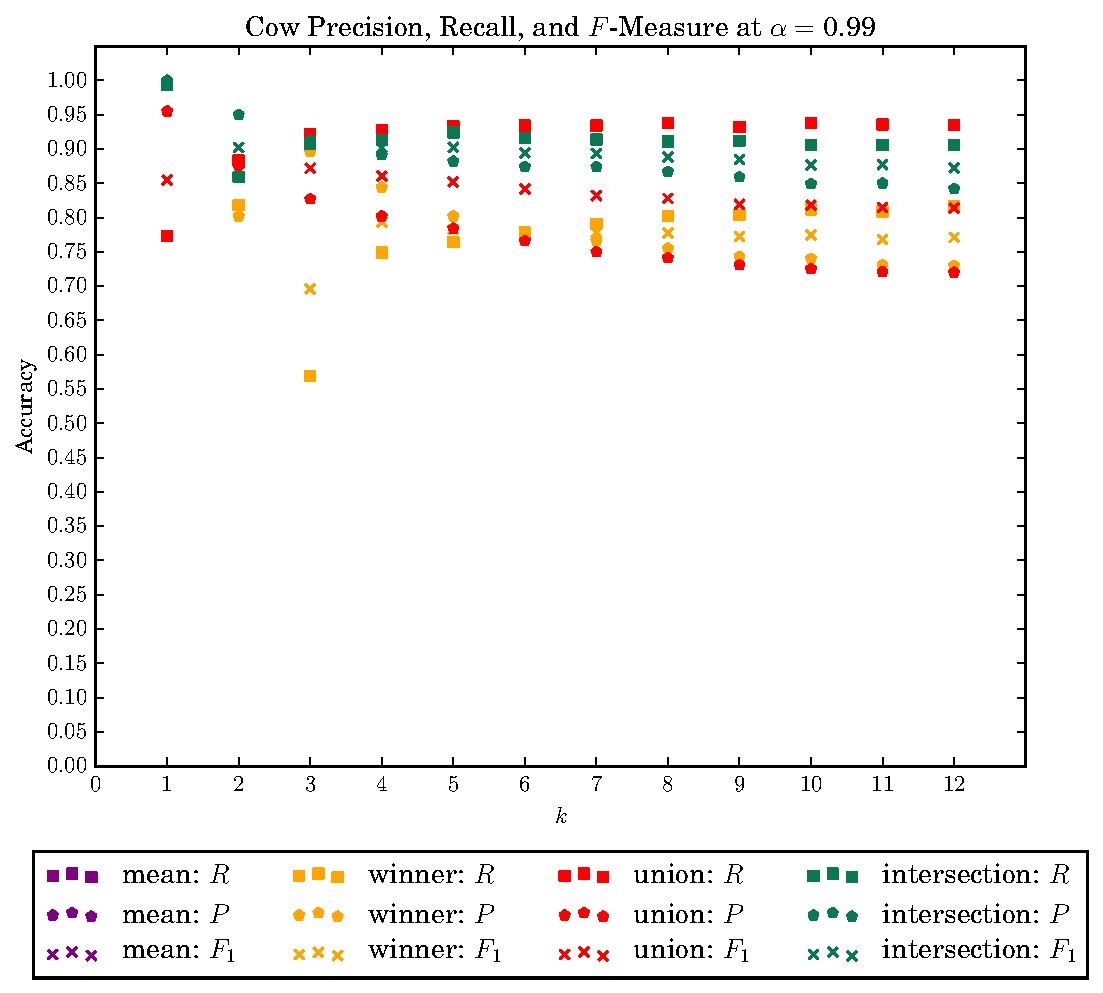
\includegraphics[width=3in]{figures/krap/Cow-ALL-metrics-12-0_990}
%\caption{There are 40 Chicken \isol{}s in CPLOP.}
%\label{fig:alpha_cow}
%\end{figure}

\begin{figure}[t]
\centering
\krapfigure{figures/krap/Cow-ALL-pvr-12-0_990}
\caption{There are 1838 Cow \isol{}s in CPLOP. Increasing the $\alpha$ for a species with this many \isol{}s made minimal improvements to the accuracy on all but the resolution by intersection algorithm, which, when compared to Figure \ref{fig:k_cow_pvr} noticeably improved.}
\label{fig:alpha_cow_pvr}
\end{figure}

Adding the $\alpha$ made minimal changes to the accuracy of Cow classifications, so only the recall versus precision is shown in Figure \ref{fig:alpha_cow_pvr}. More details into how $\alpha$ affect the classification accuracy can be seen in Tables \ref{tab:profile000}, \ref{tab:profile098}, and \ref{tab:profile099}.

%ALGORITHM
\subsection{Adjusting the Algorithm}
Choosing which algorithm to resolve the two different regions of each \isol{} is an important step. We investigate the differences between the aforementioned four algorithms as they relate to $k$ and $\alpha$ values and how each differ among species of different representation. With library-based-MST, it is important to realize the representation of a species in the library may heavily skew the accuracy of the library.

While interpreting the data, we state that there may be some ``\%'' increase or decrease which we intend to mean the increase in the raw value of the percentage.
Additionally, values in the tables represent the proportion of the three metrics, but are easily interpreted as percentages.
\autoref{sec:evaluation:krap} explains the meaning of each precision ($P$), recall ($R$), and $F$-measure ($F_1$).

\begin{table}[t]
\centering
\caption{Precision ($P$), Recall ($R$), and $F$-Measure ($F_1$) overall and for particular species at $k$=7, $\alpha=0.00$.}
\begin{tabular}{llllllll}
\cline{3-8}
                                  & \multicolumn{1}{l|}{}             & \multicolumn{3}{c|}{Meanwise}                                                  & \multicolumn{3}{c|}{Winner}                                                    \\ \hline
\multicolumn{1}{|l|}{\Spec{}} & \multicolumn{1}{l|}{$|$\Isol{}s$|$} & \multicolumn{1}{c}{$P$} & \multicolumn{1}{c}{$R$} & \multicolumn{1}{c|}{$F_1$} & \multicolumn{1}{c}{$P$} & \multicolumn{1}{c}{$R$} & \multicolumn{1}{c|}{$F_1$} \\ \hline
\multicolumn{1}{|l|}{Overall}     & \multicolumn{1}{l|}{4682}         & 0.732                   & 0.732                   & \multicolumn{1}{l|}{0.732} & 0.659                   & 0.659                   & \multicolumn{1}{l|}{0.659} \\
\multicolumn{1}{|l|}{Human}       & \multicolumn{1}{l|}{1471}         & 0.857                   & 0.922                   & \multicolumn{1}{l|}{0.888} & 0.771                   & 0.861                   & \multicolumn{1}{l|}{0.814} \\
\multicolumn{1}{|l|}{Cow}         & \multicolumn{1}{l|}{1718}         & 0.757                   & 0.885                   & \multicolumn{1}{l|}{0.816} & 0.744                   & 0.776                   & \multicolumn{1}{l|}{0.760} \\
\multicolumn{1}{|l|}{Pigeon}      & \multicolumn{1}{l|}{194}          & 0.420                   & 0.242                   & \multicolumn{1}{l|}{0.307} & 0.280                   & 0.253                   & \multicolumn{1}{l|}{0.266} \\
\multicolumn{1}{|l|}{Dog}         & \multicolumn{1}{l|}{149}          & 0.596                   & 0.436                   & \multicolumn{1}{l|}{0.504} & 0.449                   & 0.356                   & \multicolumn{1}{l|}{0.397} \\
\multicolumn{1}{|l|}{Wild Turkey} & \multicolumn{1}{l|}{72}           & 0.383                   & 0.250                   & \multicolumn{1}{l|}{0.303} & 0.277                   & 0.181                   & \multicolumn{1}{l|}{0.219} \\
\multicolumn{1}{|l|}{Chicken}     & \multicolumn{1}{l|}{40}           & 0.182                   & 0.050                   & \multicolumn{1}{l|}{0.078} & 0.143                   & 0.075                   & \multicolumn{1}{l|}{0.098} \\
\multicolumn{1}{|l|}{Cat}         & \multicolumn{1}{l|}{39}           & 0.571                   & 0.308                   & \multicolumn{1}{l|}{0.400} & 0.438                   & 0.359                   & \multicolumn{1}{l|}{0.395} \\
\multicolumn{1}{|l|}{Bat}         & \multicolumn{1}{l|}{37}           & 0.857                   & 0.973                   & \multicolumn{1}{l|}{0.911} & 0.692                   & 0.973                   & \multicolumn{1}{l|}{0.809} \\
\multicolumn{1}{|l|}{Seagull}     & \multicolumn{1}{l|}{11}           & 0.000                   & 0.000                   & \multicolumn{1}{l|}{0.000} & 0.000                   & 0.000                   & \multicolumn{1}{l|}{0.000} \\ \hline
                                  &                                   &                         &                         &                            &                         &                         &                            \\ \cline{3-8} 
                                  & \multicolumn{1}{l|}{}             & \multicolumn{3}{c|}{Union}                                                     & \multicolumn{3}{c|}{Intersection}                                              \\ \hline
\multicolumn{1}{|l|}{\Spec{}} & \multicolumn{1}{l|}{$|$\Isol{}s$|$} & \multicolumn{1}{c}{$P$} & \multicolumn{1}{c}{$R$} & \multicolumn{1}{c|}{$F_1$} & \multicolumn{1}{c}{$P$} & \multicolumn{1}{c}{$R$} & \multicolumn{1}{c|}{$F_1$} \\ \hline
\multicolumn{1}{|l|}{Overall}     & \multicolumn{1}{l|}{4682}         & 0.764                   & 0.764                   & \multicolumn{1}{l|}{0.764} & 0.747                   & 0.747                   & \multicolumn{1}{l|}{0.747} \\
\multicolumn{1}{|l|}{Human}       & \multicolumn{1}{l|}{1471}         & 0.843                   & 0.930                   & \multicolumn{1}{l|}{0.884} & 0.839                   & 0.925                   & \multicolumn{1}{l|}{0.880} \\
\multicolumn{1}{|l|}{Cow}         & \multicolumn{1}{l|}{1718}         & 0.736                   & 0.944                   & \multicolumn{1}{l|}{0.827} & 0.769                   & 0.882                   & \multicolumn{1}{l|}{0.822} \\
\multicolumn{1}{|l|}{Pigeon}      & \multicolumn{1}{l|}{194}          & 0.569                   & 0.170                   & \multicolumn{1}{l|}{0.262} & 0.470                   & 0.284                   & \multicolumn{1}{l|}{0.354} \\
\multicolumn{1}{|l|}{Dog}         & \multicolumn{1}{l|}{149}          & 0.761                   & 0.450                   & \multicolumn{1}{l|}{0.566} & 0.649                   & 0.497                   & \multicolumn{1}{l|}{0.563} \\
\multicolumn{1}{|l|}{Wild Turkey} & \multicolumn{1}{l|}{72}           & 0.688                   & 0.306                   & \multicolumn{1}{l|}{0.424} & 0.510                   & 0.361                   & \multicolumn{1}{l|}{0.423} \\
\multicolumn{1}{|l|}{Chicken}     & \multicolumn{1}{l|}{40}           & 0.000                   & 0.000                   & \multicolumn{1}{l|}{0.000} & 0.250                   & 0.100                   & \multicolumn{1}{l|}{0.143} \\
\multicolumn{1}{|l|}{Cat}         & \multicolumn{1}{l|}{39}           & 0.889                   & 0.410                   & \multicolumn{1}{l|}{0.561} & 0.571                   & 0.308                   & \multicolumn{1}{l|}{0.400} \\
\multicolumn{1}{|l|}{Bat}         & \multicolumn{1}{l|}{37}           & 0.857                   & 0.973                   & \multicolumn{1}{l|}{0.911} & 0.857                   & 0.973                   & \multicolumn{1}{l|}{0.911} \\
\multicolumn{1}{|l|}{Seagull}     & \multicolumn{1}{l|}{11}           &                      & 0.000                   & \multicolumn{1}{l|}{}   &                      & 0.000                   & \multicolumn{1}{l|}{}   \\ \hline
\end{tabular}
\label{tab:profile000}
\end{table}
Overall, with $\alpha=0.00$, Figure \ref{fig:k_overall} illustrates that the resolution by union algorithm consistently performs better. For $k=7$ and $\alpha = 0.00$, Table \ref{tab:profile000} shows that using the resolution by unions algorithm performs with 76.4\% accuracy with meanwise and resolution by winner and intersection respectively achieving 73.2\%, 65.9\%, and 74.7 accuracy\%.
Poorly represented species, like the Cat, Chicken, and Seagull did not benefit from the resolution by union algorithm, each achieving no classifications, correct or otherwise.

\begin{table}[t]
\caption{Precision ($P$), Recall ($R$), and $F$-Measure ($F_1$) overall and for particular species at $k$=7, $\alpha=0.98$.}
\begin{tabular}{lllll}
\cline{3-5}
                                    & \multicolumn{1}{l|}{}             & \multicolumn{3}{c|}{Winner} \\ \hline
\multicolumn{1}{|l|}{\Spec{}}     & \multicolumn{1}{l|}{$|$\Isol{}s$|$} & \multicolumn{1}{c}{$P$} & \multicolumn{1}{c}{$R$} & \multicolumn{1}{c|}{$F_1$} \\ \hline
\multicolumn{1}{|l|}{Overall}       & \multicolumn{1}{l|}{4682}         & 0.664 & 0.664 & \multicolumn{1}{l|}{0.664} \\
\multicolumn{1}{|l|}{Human}         & \multicolumn{1}{l|}{1471}         & 0.773 & 0.865 & \multicolumn{1}{l|}{0.816} \\
\multicolumn{1}{|l|}{Cow}           & \multicolumn{1}{l|}{1718}         & 0.749 & 0.777 & \multicolumn{1}{l|}{0.763} \\
\multicolumn{1}{|l|}{Pigeon}        & \multicolumn{1}{l|}{194}          & 0.287 & 0.254 & \multicolumn{1}{l|}{0.269} \\
\multicolumn{1}{|l|}{Dog}           & \multicolumn{1}{l|}{149}          & 0.448 & 0.349 & \multicolumn{1}{l|}{0.392} \\
\multicolumn{1}{|l|}{Wild Turkey}   & \multicolumn{1}{l|}{72}           & 0.308 & 0.222 & \multicolumn{1}{l|}{0.258} \\
\multicolumn{1}{|l|}{Chicken}       & \multicolumn{1}{l|}{40}           & 0.150 & 0.075 & \multicolumn{1}{l|}{0.100} \\
\multicolumn{1}{|l|}{Cat}           & \multicolumn{1}{l|}{39}           & 0.467 & 0.359 & \multicolumn{1}{l|}{0.406} \\
\multicolumn{1}{|l|}{Bat}           & \multicolumn{1}{l|}{37}           & 0.692 & 0.973 & \multicolumn{1}{l|}{0.809} \\
\multicolumn{1}{|l|}{Seagull}       & \multicolumn{1}{l|}{11}           & 0.000 & 0.000 & \multicolumn{1}{l|}{0.000} \\ \hline
\end{tabular}

%\centering
%\vspace{11pt}

\begin{tabular}{llllllll}
\cline{3-8}
 & \multicolumn{1}{l|}{} & \multicolumn{3}{c|}{Union} & \multicolumn{3}{c|}{Intersection} \\ \hline
\multicolumn{1}{|l|}{\Spec{}} & \multicolumn{1}{l|}{$|$\Isol{}s$|$} & \multicolumn{1}{c}{$P$} & \multicolumn{1}{c}{$R$} & \multicolumn{1}{c|}{$F_1$} & \multicolumn{1}{c}{$P$} & \multicolumn{1}{c}{$R$} & \multicolumn{1}{c|}{$F_1$} \\ \hline
\multicolumn{1}{|l|}{Overall} & \multicolumn{1}{l|}{4682} & 0.767 & 0.767 & \multicolumn{1}{l|}{0.767} & 0.780 & 0.780 & \multicolumn{1}{l|}{0.780} \\
\multicolumn{1}{|l|}{Human} & \multicolumn{1}{l|}{1471} & 0.845 & 0.930 & \multicolumn{1}{l|}{0.885} & 0.876 & 0.950 & \multicolumn{1}{l|}{0.912} \\
\multicolumn{1}{|l|}{Cow} & \multicolumn{1}{l|}{1718} & 0.742 & 0.943 & \multicolumn{1}{l|}{0.831} & 0.799 & 0.894 & \multicolumn{1}{l|}{0.844} \\
\multicolumn{1}{|l|}{Pigeon} & \multicolumn{1}{l|}{194} & 0.538 & 0.181 & \multicolumn{1}{l|}{0.271} & 0.521 & 0.333 & \multicolumn{1}{l|}{0.406} \\
\multicolumn{1}{|l|}{Dog} & \multicolumn{1}{l|}{149} & 0.756 & 0.456 & \multicolumn{1}{l|}{0.569} & 0.698 & 0.536 & \multicolumn{1}{l|}{0.606} \\
\multicolumn{1}{|l|}{Wild Turkey} & \multicolumn{1}{l|}{72} & 0.697 & 0.319 & \multicolumn{1}{l|}{0.438} & 0.571 & 0.387 & \multicolumn{1}{l|}{0.461} \\
\multicolumn{1}{|l|}{Chicken} & \multicolumn{1}{l|}{40} & 0.000 & 0.000 & \multicolumn{1}{l|}{0.000} & 0.308 & 0.121 & \multicolumn{1}{l|}{0.174} \\
\multicolumn{1}{|l|}{Cat} & \multicolumn{1}{l|}{39} & 0.889 & 0.410 & \multicolumn{1}{l|}{0.561} & 0.632 & 0.353 & \multicolumn{1}{l|}{0.453} \\
\multicolumn{1}{|l|}{Bat} & \multicolumn{1}{l|}{37} & 0.857 & 0.973 & \multicolumn{1}{l|}{0.911} & 0.878 & 0.973 & \multicolumn{1}{l|}{0.923} \\
\multicolumn{1}{|l|}{Seagull} & \multicolumn{1}{l|}{11} &  & 0.000 & \multicolumn{1}{l|}{} & 0.000 & 0.000 & \multicolumn{1}{l|}{0.000} \\ \hline
\end{tabular}



\label{tab:profile098}
\end{table}
Once we restrict with a somewhat loose threshold of 0.98, overall we see that the intersection method provides the best accuracy, improving on non-thresholded values. For $k=7$ and $\alpha=0.98$, the intersection algorithm achieves 78.0\% accuracy, while resolution by winner and union respectively achieve 66.4\% and 76.7\% accuracy.

Table \ref{tab:profile098} shows that a handful of poorly represented species achieved slightly better results when $\alpha=0.98$. Notably, the intersection algorithm $F$-measure increased slightly for Wild Turkey, Cat, and Chicken on the order of 3\%.

Unfortunately, the meanwise algorithm fails to classify when we use a large enough $\alpha$ and thus we have ommited the results in Tables \ref{tab:profile098} and \ref{tab:profile099}. In certain cells of the tables, including Table \ref{tab:profile000}, empty values in either $P$ or $F_1$ mean no classifications were made of that species.



\begin{table}[t]
\caption{Precision ($P$), Recall ($R$), and $F$-Measure ($F_1$) overall and for particular species at $k$=7, $\alpha=0.99$.}
\label{tab:profile099}
\begin{tabular}{lllll}
\cline{3-5}
                                  & \multicolumn{1}{l|}{}           & \multicolumn{3}{l|}{Winner}                \\ \hline
\multicolumn{1}{|l|}{\Spec{}} & \multicolumn{1}{l|}{$|$\Isol{}s$|$} & \multicolumn{1}{c|}{$P$}   & \multicolumn{1}{c|}{$R$}   & \multicolumn{1}{l|}{$F_1$} \\ \hline
\multicolumn{1}{|l|}{Overall}     & \multicolumn{1}{l|}{4682}            & 0.680 & 0.680 & \multicolumn{1}{l|}{0.680} \\
\multicolumn{1}{|l|}{Human}       & \multicolumn{1}{l|}{1471}            & 0.780 & 0.872 & \multicolumn{1}{l|}{0.823} \\
\multicolumn{1}{|l|}{Cow}         & \multicolumn{1}{l|}{1718}            & 0.766 & 0.791 & \multicolumn{1}{l|}{0.778} \\
\multicolumn{1}{|l|}{Pigeon}      & \multicolumn{1}{l|}{194}             & 0.314 & 0.263 & \multicolumn{1}{l|}{0.286} \\
\multicolumn{1}{|l|}{Dog}         & \multicolumn{1}{l|}{149}             & 0.527 & 0.401 & \multicolumn{1}{l|}{0.455} \\
\multicolumn{1}{|l|}{Wild Turkey} & \multicolumn{1}{l|}{72}              & 0.320 & 0.222 & \multicolumn{1}{l|}{0.262} \\
\multicolumn{1}{|l|}{Chicken}     & \multicolumn{1}{l|}{40}              & 0.167 & 0.100 & \multicolumn{1}{l|}{0.125} \\
\multicolumn{1}{|l|}{Cat}         & \multicolumn{1}{l|}{39}              & 0.433 & 0.333 & \multicolumn{1}{l|}{0.376} \\
\multicolumn{1}{|l|}{Bat}         & \multicolumn{1}{l|}{37}              & 0.720 & 0.973 & \multicolumn{1}{l|}{0.828} \\
\multicolumn{1}{|l|}{Seagull}     & \multicolumn{1}{l|}{11}              & 0.429 & 0.273 & \multicolumn{1}{l|}{0.334} \\ \hline
\end{tabular}

%\vspace{11pt}
%\centering

\begin{tabular}{llllllll}
\cline{3-8}
                                  & \multicolumn{1}{c|}{}             & \multicolumn{3}{c|}{Union}                 & \multicolumn{3}{c|}{Intersection}          \\ \hline
\multicolumn{1}{|l|}{\Spec{}} & \multicolumn{1}{l|}{$|$\Isol{}s$|$} & \multicolumn{1}{c|}{$P$}   & \multicolumn{1}{c|}{$R$}   & \multicolumn{1}{c|}{$F_1$} & \multicolumn{1}{c|}{$P$}   & \multicolumn{1}{c|}{$R$}   & \multicolumn{1}{l|}{$F_1$} \\ \hline
\multicolumn{1}{|l|}{Overall}     & \multicolumn{1}{l|}{4682}         & 0.766 & 0.766 & \multicolumn{1}{l|}{0.766} & 0.859 & 0.859 & \multicolumn{1}{l|}{0.859} \\
\multicolumn{1}{|l|}{Human}       & \multicolumn{1}{l|}{1471}         & 0.843 & 0.925 & \multicolumn{1}{l|}{0.882} & 0.926 & 0.979 & \multicolumn{1}{l|}{0.952} \\
\multicolumn{1}{|l|}{Cow}         & \multicolumn{1}{l|}{1718}         & 0.750 & 0.934 & \multicolumn{1}{l|}{0.832} & 0.874 & 0.914 & \multicolumn{1}{l|}{0.894} \\
\multicolumn{1}{|l|}{Pigeon}      & \multicolumn{1}{l|}{194}          & 0.476 & 0.205 & \multicolumn{1}{l|}{0.287} & 0.611 & 0.468 & \multicolumn{1}{l|}{0.530} \\
\multicolumn{1}{|l|}{Dog}         & \multicolumn{1}{l|}{149}          & 0.739 & 0.456 & \multicolumn{1}{l|}{0.564} & 0.838 & 0.738 & \multicolumn{1}{l|}{0.785} \\
\multicolumn{1}{|l|}{Wild Turkey} & \multicolumn{1}{l|}{72}           & 0.719 & 0.319 & \multicolumn{1}{l|}{0.442} & 0.667 & 0.455 & \multicolumn{1}{l|}{0.541} \\
\multicolumn{1}{|l|}{Chicken}     & \multicolumn{1}{l|}{40}           & 0.000 & 0.000 & \multicolumn{1}{l|}{0.000} & 0.000 & 0.000 & \multicolumn{1}{l|}{0.000} \\
\multicolumn{1}{|l|}{Cat}         & \multicolumn{1}{l|}{39}           & 0.938 & 0.385 & \multicolumn{1}{l|}{0.546} & 0.909 & 0.588 & \multicolumn{1}{l|}{0.714} \\
\multicolumn{1}{|l|}{Bat}         & \multicolumn{1}{l|}{37}           & 0.837 & 0.973 & \multicolumn{1}{l|}{0.900} & 0.973 & 1.000 & \multicolumn{1}{l|}{0.986} \\
\multicolumn{1}{|l|}{Seagull}     & \multicolumn{1}{l|}{11}           & 0.000 & 0.000 & \multicolumn{1}{l|}{0.000} &    & 0.000 & \multicolumn{1}{l|}{}   \\ \hline
\end{tabular}
\end{table}
Restricting with $\alpha=0.99$, our definition of strain differentiation, overall accuracy improves more with resolution by intersection and less so with resolutions by winner and union, garnering 85.9\%, 68.0\%, and 76.6\% accuracy respectively. Again, meanwise resolution fails to produce any classifications.

For poorly represented species, we see some similar improvements for $P$, $R$, and $F_1$, but also some exceptions. Wild Turkey for example, improves by about 2\%-3\% for resolutions by winner and union and 11\% for resolution by intersection, while Cat decreases by 3\% for resolution by winner, but improves by 6\% and 47\% for resolution by union and intersection.

\subsection{Underrepresented Species}
\begin{figure}[t]
\centering
\krapfigure{figures/krap/Chicken-ALL-metrics-12-0_000}
\caption{There are 40 Chicken \isol{}s in CPLOP. Unfortunately, due to their low representation in CPLOP, classification accuracy is low.}
\label{fig:k_chicken}
\end{figure}
Some species had worse accuracy than the overall accuracy. In particular, species such as Chicken with only 40 \isol{}s representing it showed similar leveling of accuracy for $k>5$, but had far poorer accuracy, as shown in Figure \ref{fig:k_chicken}. For $k>5$, the accuracy of classifying chicken ranges from as low as 10\% to a peak of 26\%. The classification accuracy for many species in CPLOP heavily relies on its representation in CPLOP.

One notable exception is the Bat. In everyone application of our \kNN{} algorithms, Bat has above 95\% accuracy. It is possible that due to their small size and relative dietary segregation from the surrounding environment that the strains of \ecoli{} stay particularly unique. It may also be a quirk of the fact that each \isol{} comes from a single \host{}, making it difficult to draw conclusions from such results.
